\documentclass[12pt, titlepage]{article}

\usepackage{fullpage}
\usepackage[round]{natbib}
\usepackage{multirow}
\usepackage{booktabs}
\usepackage{tabularx}
\usepackage{graphicx}
\usepackage{float}
\usepackage{hyperref}
\hypersetup{
    colorlinks,
    citecolor=blue,
    filecolor=black,
    linkcolor=red,
    urlcolor=blue
}

%%% Comments

\usepackage{color}

\newif\ifcomments\commentstrue %displays comments
%\newif\ifcomments\commentsfalse %so that comments do not display

\ifcomments
\newcommand{\authornote}[3]{\textcolor{#1}{[#3 ---#2]}}
\newcommand{\todo}[1]{\textcolor{red}{[TODO: #1]}}
\else
\newcommand{\authornote}[3]{}
\newcommand{\todo}[1]{}
\fi

\newcommand{\wss}[1]{\authornote{blue}{SS}{#1}} 
\newcommand{\plt}[1]{\authornote{magenta}{TPLT}{#1}} %For explanation of the template
\newcommand{\an}[1]{\authornote{cyan}{Author}{#1}}

\newcommand{\progname}{SmartServe} % PUT YOUR PROGRAM NAME HERE
\newcommand{\authname}{Team 21, StoneCap Solutions
\\ Max Turek $turekm$
\\ Ryan Were $werer$
\\ Sam Nusselder $nusselds$
\\ Peter Minbashian $minbashp$
\\ David Bednar $bednad1$} % AUTHOR NAMES                    

\usepackage{hyperref}
    \hypersetup{colorlinks=true, linkcolor=blue, citecolor=blue, filecolor=blue,
                urlcolor=blue, unicode=false}
    \urlstyle{same}

\newcounter{acnum}
\newcommand{\actheacnum}{AC\theacnum}
\newcommand{\acref}[1]{AC\ref{#1}}

\newcounter{ucnum}
\newcommand{\uctheucnum}{UC\theucnum}
\newcommand{\uref}[1]{UC\ref{#1}}

\newcounter{mnum}
\newcommand{\mthemnum}{M\themnum}
\newcommand{\mref}[1]{M\ref{#1}}

\begin{document}

\title{Module Guide for \progname{}} 
\author{\authname}
\date{\today}

\maketitle

\pagenumbering{roman}

\section{Revision History}

\begin{tabularx}{\textwidth}{| s | s | s | X |}
        \toprule
        \textbf{Version} & \textbf{Date} & \textbf{Developer(s)} & \textbf{Change(s)}\\
        \midrule
         & & Max Turek & \\
         & & Ryan Were & \\
        1.0 & 01/18/23 & Sam Nusselder & Initial Draft\\
         & & Peter Minbashian & \\ 
         & & David Bednar & \\ 
        \bottomrule
        \hline
\end{tabularx}

\newpage

\section{Reference Material}

\subsection{Abbreviations and Acronyms}

\renewcommand{\arraystretch}{1.2}
  \toprule		
  \textbf{symbol} & \textbf{description}\\
  \midrule \\
  AC & Anticipated Change\\
  DAG & Directed Acyclic Graph \\
  M & Module \\
  MG & Module Guide \\
  OS & Operating System \\
  R & Requirement\\
  SC & Scientific Computing \\
  SRS & Software Requirements Specification\\
  \progname & Explanation of program name\\
  UC & Unlikely Change \\

\newpage

\tableofcontents

\listoftables

\listoffigures

\newpage

\pagenumbering{arabic}

\section{Introduction}

Decomposing a system into modules is a commonly accepted approach to developing
software.  A module is a work assignment for a programmer or programming
team~\citep{ParnasEtAl1984}.  We advocate a decomposition
based on the principle of information hiding~\citep{Parnas1972a}.  This
principle supports design for change, because the ``secrets'' that each module
hides represent likely future changes.  Design for change is valuable in SC,
where modifications are frequent, especially during initial development as the
solution space is explored.  

Our design follows the rules layed out by \citet{ParnasEtAl1984}, as follows:
\begin{itemize}
\item System details that are likely to change independently should be the
  secrets of separate modules.
\item Each data structure is implemented in only one module.
\item Any other program that requires information stored in a module's data
  structures must obtain it by calling access programs belonging to that module.
\end{itemize}

After completing the first stage of the design, the Software Requirements
Specification (SRS), the Module Guide (MG) is developed. The MG
specifies the modular structure of the system and is intended to allow both
designers and maintainers to easily identify the parts of the software.  The
potential readers of this document are as follows:

\begin{itemize}
\item New project members: This document can be a guide for a new project member
  to easily understand the overall structure and quickly find the
  relevant modules they are searching for.
\item Maintainers: The hierarchical structure of the module guide improves the
  maintainers' understanding when they need to make changes to the system. It is
  important for a maintainer to update the relevant sections of the document
  after changes have been made.
\item Designers: Once the module guide has been written, it can be used to
  check for consistency, feasibility, and flexibility. Designers can verify the
  system in various ways, such as consistency among modules, feasibility of the
  decomposition, and flexibility of the design.
\end{itemize}

The rest of the document is organized as follows. Section
requirements. Section \ref{SecMH} summarizes the module decomposition that
was constructed according to the likely changes. Section \ref{SecConnection}
specifies the connections between the software requirements and the
modules. Section \ref{SecMD} gives a detailed description of the
modules. Section \ref{SecTM} includes two traceability matrices. One checks
the completeness of the design against the requirements provided in the SRS. The
other shows the relation between anticipated changes and the modules. Section
\ref{SecUse} describes the use relation between modules.

\section{Anticipated and Unlikely Changes} \label{SecChange}

This section lists possible changes to the system. According to the likeliness
of the change, the possible changes are classified into two
categories. Anticipated changes are listed in Section \ref{SecAchange}, and
unlikely changes are listed in Section \ref{SecUchange}.

\subsection{Anticipated Changes} \label{SecAchange}

\begin{description}
\item[\refstepcounter{acnum} \actheacnum \label{acHardware}:] Instead of using an API for login functionality we will use the Raspberry Pi as a host for user login functionality
\item [Rational:] This anticipated change is expected for two reasons. Firstly, it becomes easier for the design if all processes are done through the pi. Also, it is cheaper as hosting anything externally costs money.
\item[\refstepcounter{acnum} \actheacnum \label{acInput}:] Drink volumes may now be calculated via a number of drinks made with certain ingredients to find volumes rather than using sensors
\item [Rational:] This anticipated change is expected for to both reduce costs, as less sensor will be required for the project and to make the functionality simpler as it would be easier to design and require less processing power from the pi.
\end{description}

\subsection{Unlikely Changes} \label{SecUchange}

The module design should be as general as possible. However, a general system is
more complex. Sometimes this complexity is not necessary. Fixing some design
decisions at the system architecture stage can simplify the software design. If
these decision should later need to be changed, then many parts of the design
will potentially need to be modified. Hence, it is not intended that these
decisions will be changed.

\begin{description}
\item[\refstepcounter{ucnum} \uctheucnum \label{ucIO}:] All drink order data will be saved in a database
\item [Rational:] Too complex to implement and the manager can supervise

\item[\refstepcounter{ucnum} \uctheucnum \label{ucIO}:] Personalized drink recommendation feature is implemented
\item [Rational:] Too complex to implement and the manager can supervise usage of machine for any safety concerns around under age people using the machine 

\item[\refstepcounter{ucnum} \uctheucnum \label{ucIO}:] Face ID recognition is required for all users before order confirmation
\item [Rational:] Too complex to implement and the Pi would not have enough processing power

\item[\refstepcounter{ucnum} \uctheucnum \label{ucIO}:] Custom drink creation feature is implemented
\item [Rational:] People could make drinks which exceed appropriate alcohol limits

\item[\refstepcounter{ucnum} \uctheucnum \label{ucIO}:] Social media sharing options for all drinks
\item [Rational:] Too complex to implement and the Pi would not have enough processing power

\item[\refstepcounter{ucnum} \uctheucnum \label{ucIO}:] Drink discussion forum feature
\item [Rational:] This would require a lot of data storage and far too much processing power for current supplies
\item[\refstepcounter{ucnum} \uctheucnum \label{ucIO}:] Drink review feature on individual drinks
\item [Rational:] This would more data storage resulting in total usage going beyond what is currently available for the entire system
\item[\refstepcounter{ucnum} \uctheucnum \label{ucIO}:] Sliced lemon or lime add-on option for all orders
\item [Rational:] Too complex to integrate into design and presents risk of poor maintenance resulting in expired food

\end{description}

\section{Module Hierarchy} \label{SecMH}

This section provides an overview of the module design. Modules are summarized
in a hierarchy decomposed by secrets in Table \ref{TblMH}. The modules listed
below, which are leaves in the hierarchy tree, are the modules that will
actually be implemented.

\begin{description}
\item [\refstepcounter{mnum} \mthemnum \label{mHH}:] Python Hardware Module
\item [\refstepcounter{mnum} \mthemnum \label{mHH}:] 
Send Order Module
\item [\refstepcounter{mnum} \mthemnum \label{mHH}:] 
Volume Tracker Module
\item [\refstepcounter{mnum} \mthemnum \label{mHH}:] 
Drink Ready
\item [\refstepcounter{mnum} \mthemnum \label{mHH}:] Menu Page Module
\item [\refstepcounter{mnum} \mthemnum \label{mHH}:] Admin Ingredient Input Module
\item [\refstepcounter{mnum} \mthemnum \label{mHH}:] Order History Module
\item [\refstepcounter{mnum} \mthemnum \label{mHH}:] Header Module
\item [\refstepcounter{mnum} \mthemnum \label{mHH}:] Login Page Module
\end{description}


\begin{table}[h!]
\centering
\begin{tabular}{p{0.3\textwidth} p{0.6\textwidth}}
\toprule
\textbf{Level 1} & \textbf{Level 2}\\
\midrule

{Hardware-Hiding Module} & Python Hardware Module \\
\midrule

\multirow{3}{0.3\textwidth}{Behaviour-Hiding Module}
& Send Order\\
& Volume Tracker\\
& Drink Ready\\
\midrule

\multirow{3}{0.3\textwidth}{Software Decision Module}
& Menu Page\\
& Admin Ingredient Input\\
& Order History\\
& Header\\
& Login Page\\
\bottomrule

\end{tabular}
\caption{Module Hierarchy}
\label{TblMH}
\end{table}

\section{Connection Between Requirements and Design} \label{SecConnection}

The design of the system is intended to satisfy the requirements developed in
the SRS. In this stage, the system is decomposed into modules. The connection
between requirements and modules is listed in Table~\ref{TblRT}.

\section{Module Decomposition} \label{SecMD}

Only the leaf modules in the hierarchy have to be implemented. If a dash
(\emph{--}) is shown, this means that the module is not a leaf and will not have
to be implemented.

\subsection{Python Hardware Module}
\begin{description}
\item[Secrets:]A boolean value corresponding to the creation of a drink
\item[Services:]Serves to give insight as to when the drink is complete after, all ingredients have been poured, and the machine is ready to begin the next drink
\item[Implemented By: OS and Web Sockets]
\end{description}

\subsection{Send Order}
\begin{description}
\item[Secrets:]JSON Data types and NodeJS Server Environment (Hosted on Rasberry Pi)
\item[Services:]Module is used to send drink orders made by customers to Smart Serve Hardware to prompt the hardware to begin making said drink. Data consists of GPIO pin numbers to activate along with a coupling number to correspond with how long the pin should be activated.
\item[Implemented By:]OS
\end{description}

\subsection{Volume Tracker}
\begin{description}
\item[Secrets:]The contents of the required behaviors.
\item[Services:]Module is used to track the amount of liquid of ingredients left within the system. Anytime a drink has been ordered, the system should use the volume tracker to update the amount of volume it has for each drink.
\item[Implemented By]: OS
 \end{description}

 \subsection{Drink Ready}
\begin{description}
\item[Secrets:]A boolean value corresponding to the completion of a drink sent from the Hardware
\item[Services:]This Module serves as the purpose to notify the user once their drink has been finished. This message will consist of a pop up window for the user on their device when on the web app.
\item[Implemented By]: OS
 \end{description}

\subsection{Login Page Module}

\begin{description}
\item[Secrets:] The login module contains a database of usernames and corresponding passwords. The module also contains functions and variables used to sign in and register users.
\item[Services:] Users will be granted access to the header module when the sign-in or register processes are successful.
\item[Implemented By:] OS and Database (MySQl)
\end{description}

\subsection{Menu Page Module}

\begin{description}
\item[Secrets:] The Menu Page Module consists of a main list containing all available drinks. Each drink contains a name, image, category, and JSON object of ingredients and ingredient sizes.
\item[Services:] Users will be able to see the list of all available drinks to select from. Users will be able to send orders to the send order module to begin the process of making their drink.
\item[Implemented By:] OS
\end{description}

\subsection{Header Page Module}

\begin{description}
\item[Secrets:] The Header Page Module contains the current users' username and a database of administrative users.
\item[Services:] Users will be able to navigate to either the menu page, the admin ingredient input, or the order history module
\item[Implemented By:] OS
\end{description}

\subsection{Admin Ingredient Input Module}

\begin{description}
\item[Secrets:] The Admin Ingredient Input Module contains a list of ingredients and corresponding dispenser locations.
\item[Services:] Admin users will be able to input ingredients and corresponding dispenser locations. The menu page drink database is filled with available ingredients from the current module.
\item[Implemented By:] OS and Database (MySQl)
\end{description}

\subsection{Order History Module}

\begin{description}
\item[Secrets:] The Order History Module contains a list of all drinks ordered since the web application has been running.
\item[Services:] Users will be able to get access and view their entire order history through a vizualization methods such as histograms and pie charts.
\item[Implemented By:] Database (MySQl)
\end{description}


\section{Traceability Matrix} \label{SecTM}

This section shows two traceability matrices: between the modules and the
requirements and between the modules and the anticipated changes.

% the table should use mref, the requirements should be named, use something
% like fref
\begin{table}[H]
\centering
\begin{tabular}{p{0.2\textwidth} p{0.6\textwidth}}
\toprule
\textbf{Req.} & \textbf{Modules}\\
\midrule
ODR2 & M2, M5, M8\\
ODR5 & M3, M5, M6\\
ODR6 & M1, M4 \\
ODR9 & M6 \\
ODR10 & M6\\
ODR12 & M7\\
ODR14 & M1 \\
ODR15 & M9\\
ODR16 & M6, M9\\
UHR4 & M5\\
MSR4 & M6\\
LR3 & M6\\
LFR1 & M6, M7, M8, M9\\
PR2 & M6, M7, M8, M9\\
\bottomrule
\end{tabular}
\caption{Trace Between Requirements and Modules}
\label{TblRT}
\end{table}

\begin{table}[H]
\centering
\begin{tabular}{p{0.2\textwidth} p{0.6\textwidth}}
\toprule
\textbf{AC} & \textbf{Modules}\\
\midrule
AC1 & M2 \\
AC2 & M5 \\
\bottomrule
\end{tabular}
\caption{Trace Between Anticipated Changes and Modules}
\label{TblACT}
\end{table}

\section{Use Hierarchy Between Modules} \label{SecUse}



\begin{figure}[H]
\centering
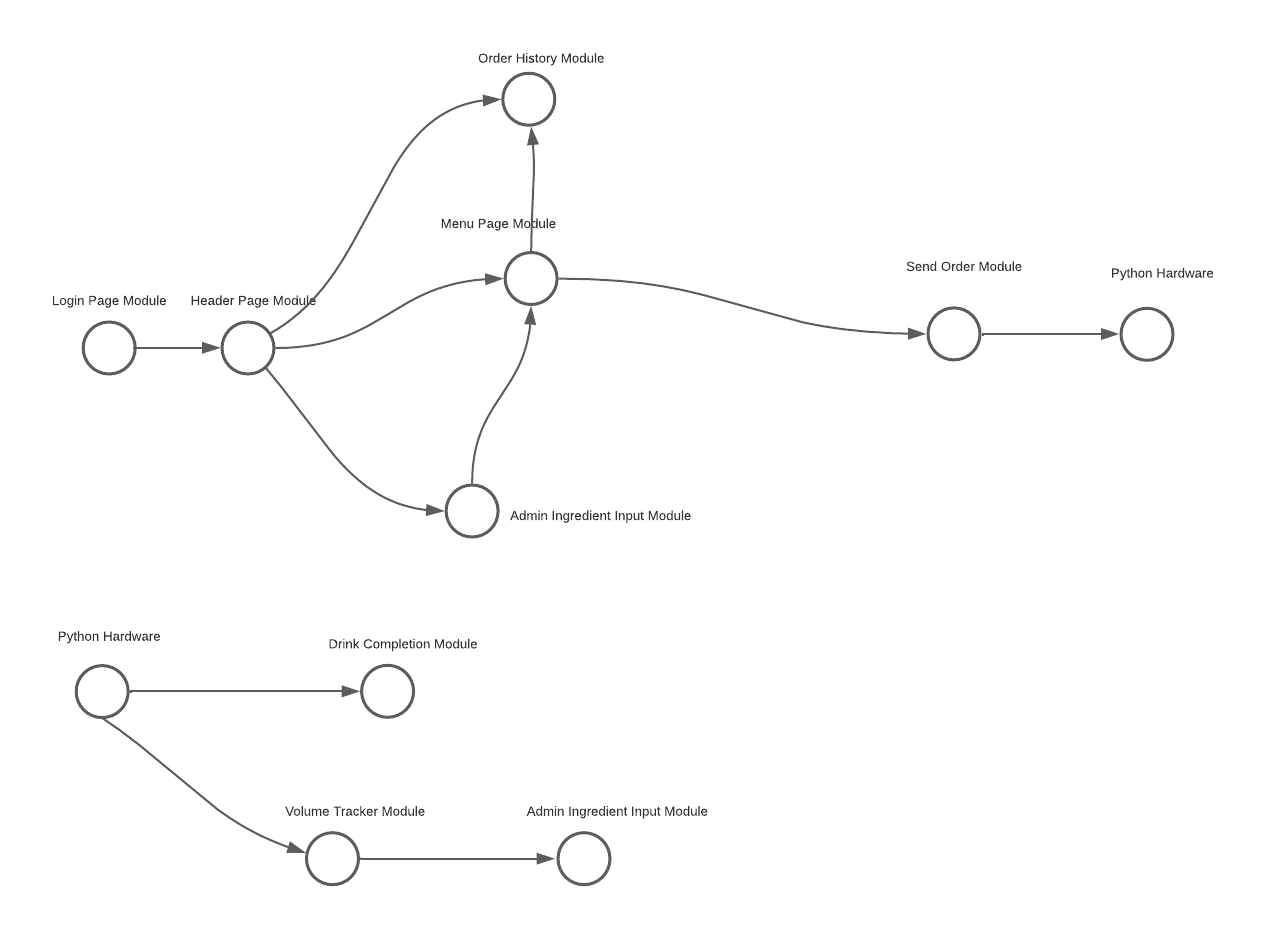
\includegraphics[width=0.7\textwidth]{Blank board.png}
\caption{Use hierarchy from the web application to the hardware}
\caption{Use hierarchy from the hardware to the web application}
\label{FigUH}
\end{figure}

%\section*{References}

\bibliographystyle {plainnat}
\bibliography{../../../refs/References}

\end{document}
